\PassOptionsToPackage{unicode}{hyperref}
\documentclass[aspectratio=1610, professionalfonts, 9pt, hyperref={colorlinks=false}]{beamer}

\usefonttheme[onlymath]{serif}
\usetheme[showtotalframes]{tudo}

\ifluatex
  \usepackage{polyglossia}
  \setmainlanguage{german}
\else
  \ifxetex
    \usepackage{polyglossia}
    \setmainlanguage{german}
  \else
    \usepackage[german]{babel}
  \fi
\fi
    

% Mathematik
\usepackage{amsmath}
\usepackage{amssymb}
\usepackage{mathtools}
\usepackage{cancel}


\usepackage{hyperref}

\usepackage{bookmark}

% Biber
\usepackage[style=numeric-comp,backend=bibtex,sorting=none]{biblatex}
\addbibresource{references.bib}
\DefineBibliographyStrings{german}{andothers = {{et\,al\adddot}}}

% SI UNITX

\usepackage[
  locale=DE,                 % deutsche Einstellungen
  separate-uncertainty=true, % immer Fehler mit \pm
  per-mode=reciprocal,       % ^-1 für inverse Einheiten
  % alternativ:
  % per-mode=reciprocal, % m s^{-1}
  % decimal-marker=., % . statt , f�r Dezimalzahlen
]{siunitx}

%%%%%%%%%%%%%%%%%%%%%%%%%%%%%%%%%%%%%%%%%%%%%%%%%%%%%%%%%%%%%%%%%%%%%%%%%%%%%%%%
%%%%%-------------Hier Titel/Autor/Grafik/Lehrstuhl eintragen--------------%%%%%
%%%%%%%%%%%%%%%%%%%%%%%%%%%%%%%%%%%%%%%%%%%%%%%%%%%%%%%%%%%%%%%%%%%%%%%%%%%%%%%%

%Titel:
\title{Von der Entdeckung der kosmischen Strahlung bis zu modernen Luftschauerexperimenten}
%Autor
\author[J.~Alameddine]{Jean-Marco Alameddine}
%Lehrstuhl/Fakultät
\institute[Lehrstuhl E5b]{Lehrstuhl E5b \\  Fakultät Physik}
%Titelgrafik 
%\titlegraphic{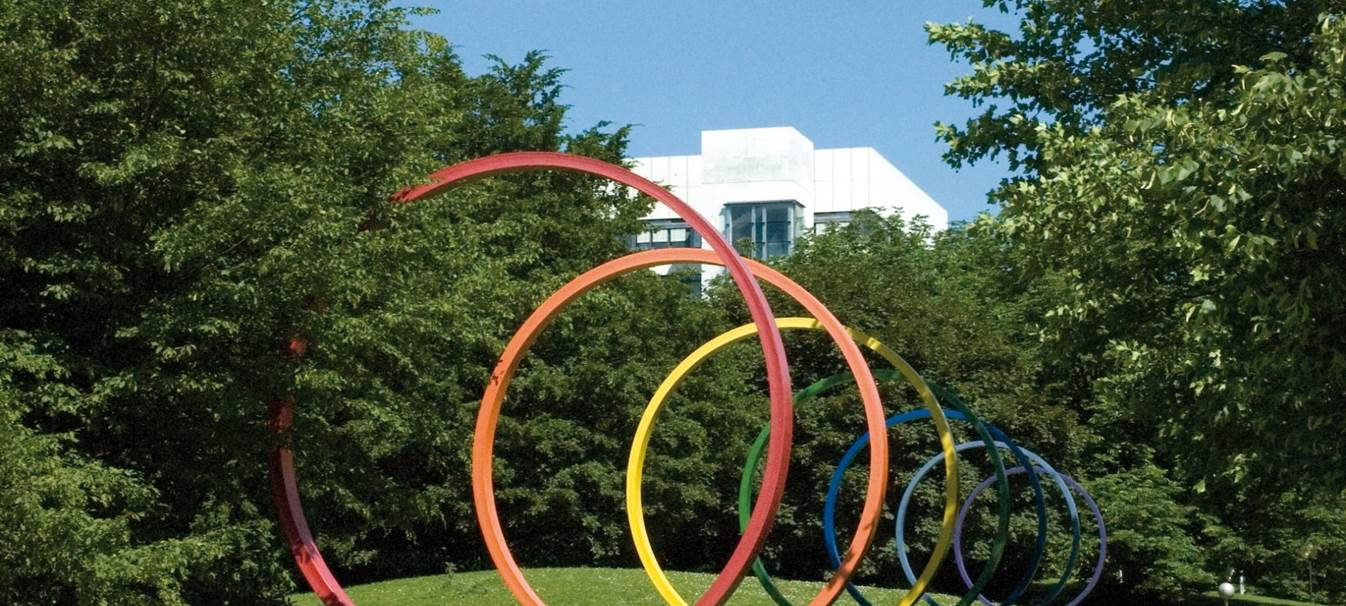
\includegraphics[width=0.7\textwidth]{images/tudo-title-2.jpg}}


\begin{document}

\maketitle



\begin{frame}
    Ende 19. Jahrhundert: "Die Physik ist als Wissenschaft abgeschlossen..."
    \begin{figure}
        \includegraphics<2>[width=0.23\textwidth]{images/first_xray.jpg} 
        \only<2->{\cite{xray}}
        \hfill
        \includegraphics<2>[width=0.4\textwidth]{images/Becquerel_plate.jpg} 
        \only<2->{\cite{radio}}
        \hfill
        \includegraphics<2>[width=0.23\textwidth]{images/Max_Planck_(1858-1947).jpg}
        \only<2->{\cite{planck}}
    \end{figure}
\end{frame} 


\begin{frame}{Der Weg zur kosmischen Höhenstrahlung...}
  \begin{columns}
    \column{0.6\textwidth}
      \begin{itemize}
        \setlength\itemsep{0.5em}
        \item Bereits früh bekannt (Coulomb, 1785): Ein isolierter elektrischer Leiter verliert mit der Zeit seine Ladung
        \item [$\rightarrow$] Leitfähigkeit der Luft?
        \item Elster und Geitel (siehe Abbildung) 1900 mit der Hypothese:
        \item [$\rightarrow$] Kleinste Mengen radioaktiver Substanzen in der Luft und in der Erde, welche der Luft ihre Leitfähigkeit verleihen
        \item Erste Untersuchungen von Ionisation außerhalb von Laboren (Höhlen, Salzminen...)
      \end{itemize}
        \vspace*{10px}
  
    \column{0.4\textwidth}
      \begin{figure}
          \centering
          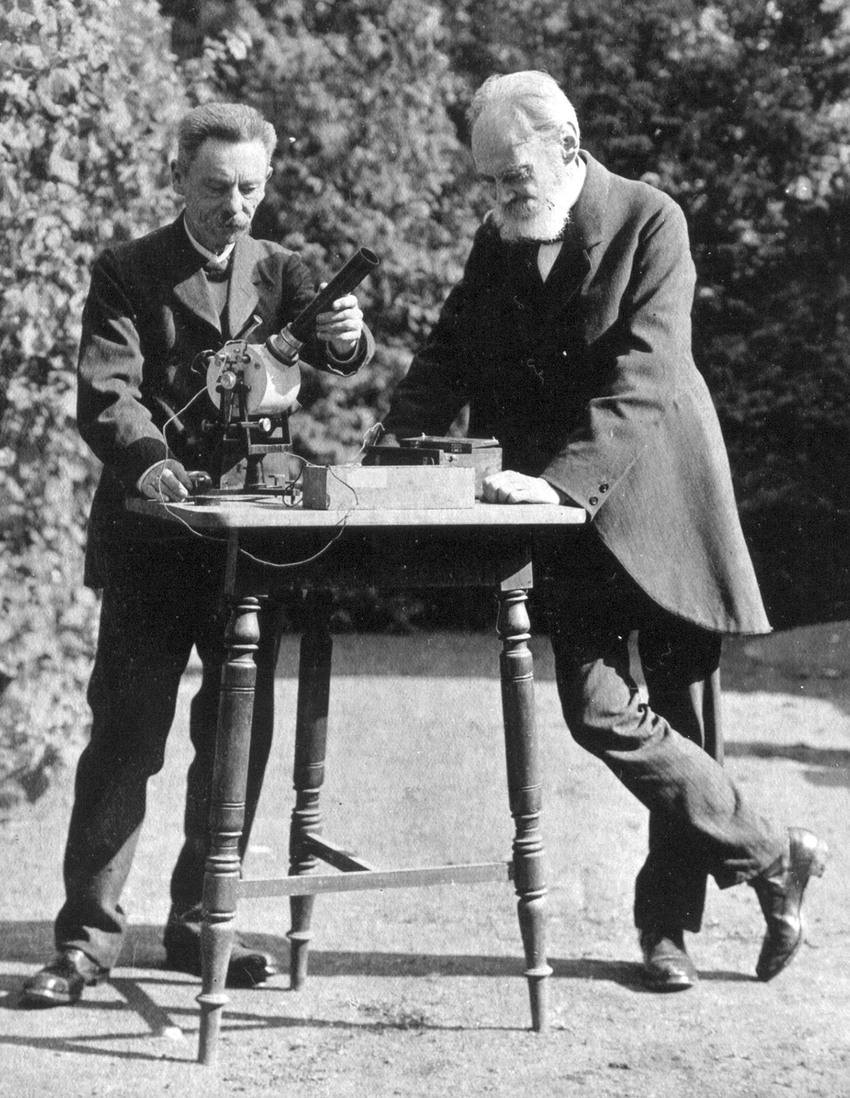
\includegraphics[width=0.7\linewidth]{images/Julius-Elster-and-Hans-Geitel-experimenting-in-the-garden-of-Elsters-house-The.png}
          \caption{Julius Elster und Hans Geitel \cite{article}}
      \end{figure}
  \end{columns}
\end{frame}

\begin{frame}{Erste Untersuchungen der Ionisation in der Höhe}
      \begin{itemize}
        \setlength\itemsep{0.5em}
        \item Erste Messungen der Ionisation (mithilfe eines Elektroskopes) in der Höhe:
        \item[$\rightarrow$] \textbf{1910}: Theodor Wulf, Messung auf dem Eiffelturm ($h \approx \SI{300}{\metre}$)  
        \item[$\rightarrow$] \textbf{1909-1911}: Albert Gockel, Ballonflüge in der Schweiz ($h \lesssim \SI{4500}{\metre}$)
      \end{itemize}
        \vspace*{10px}

        $\Rightarrow$ Deutlich geringere Abnahme der Ionisationsstärke mit der Höhe als angenommen 
\end{frame}

\begin{frame}{}
  \begin{columns}
    \column{0.5\textwidth}
      \begin{itemize}
        \setlength\itemsep{0.5em}
        \item Victor Hess, arbeitete ab 1910 am "Institut für Radiumforschung" in Wien
        \item Durchmessung von Untersuchungen der Absorption von \gamma-Strahlung in Luft
        \item [$\rightarrow$] Schlussfolgerung aus Messungen: In \SI{500}{\metre} Höhe würde die Strahlung der Erde auf wenige Prozent abgefallen sein
      \end{itemize}
        \vspace*{10px}
  
    \column{0.5\textwidth}
      \begin{figure}
          \centering
          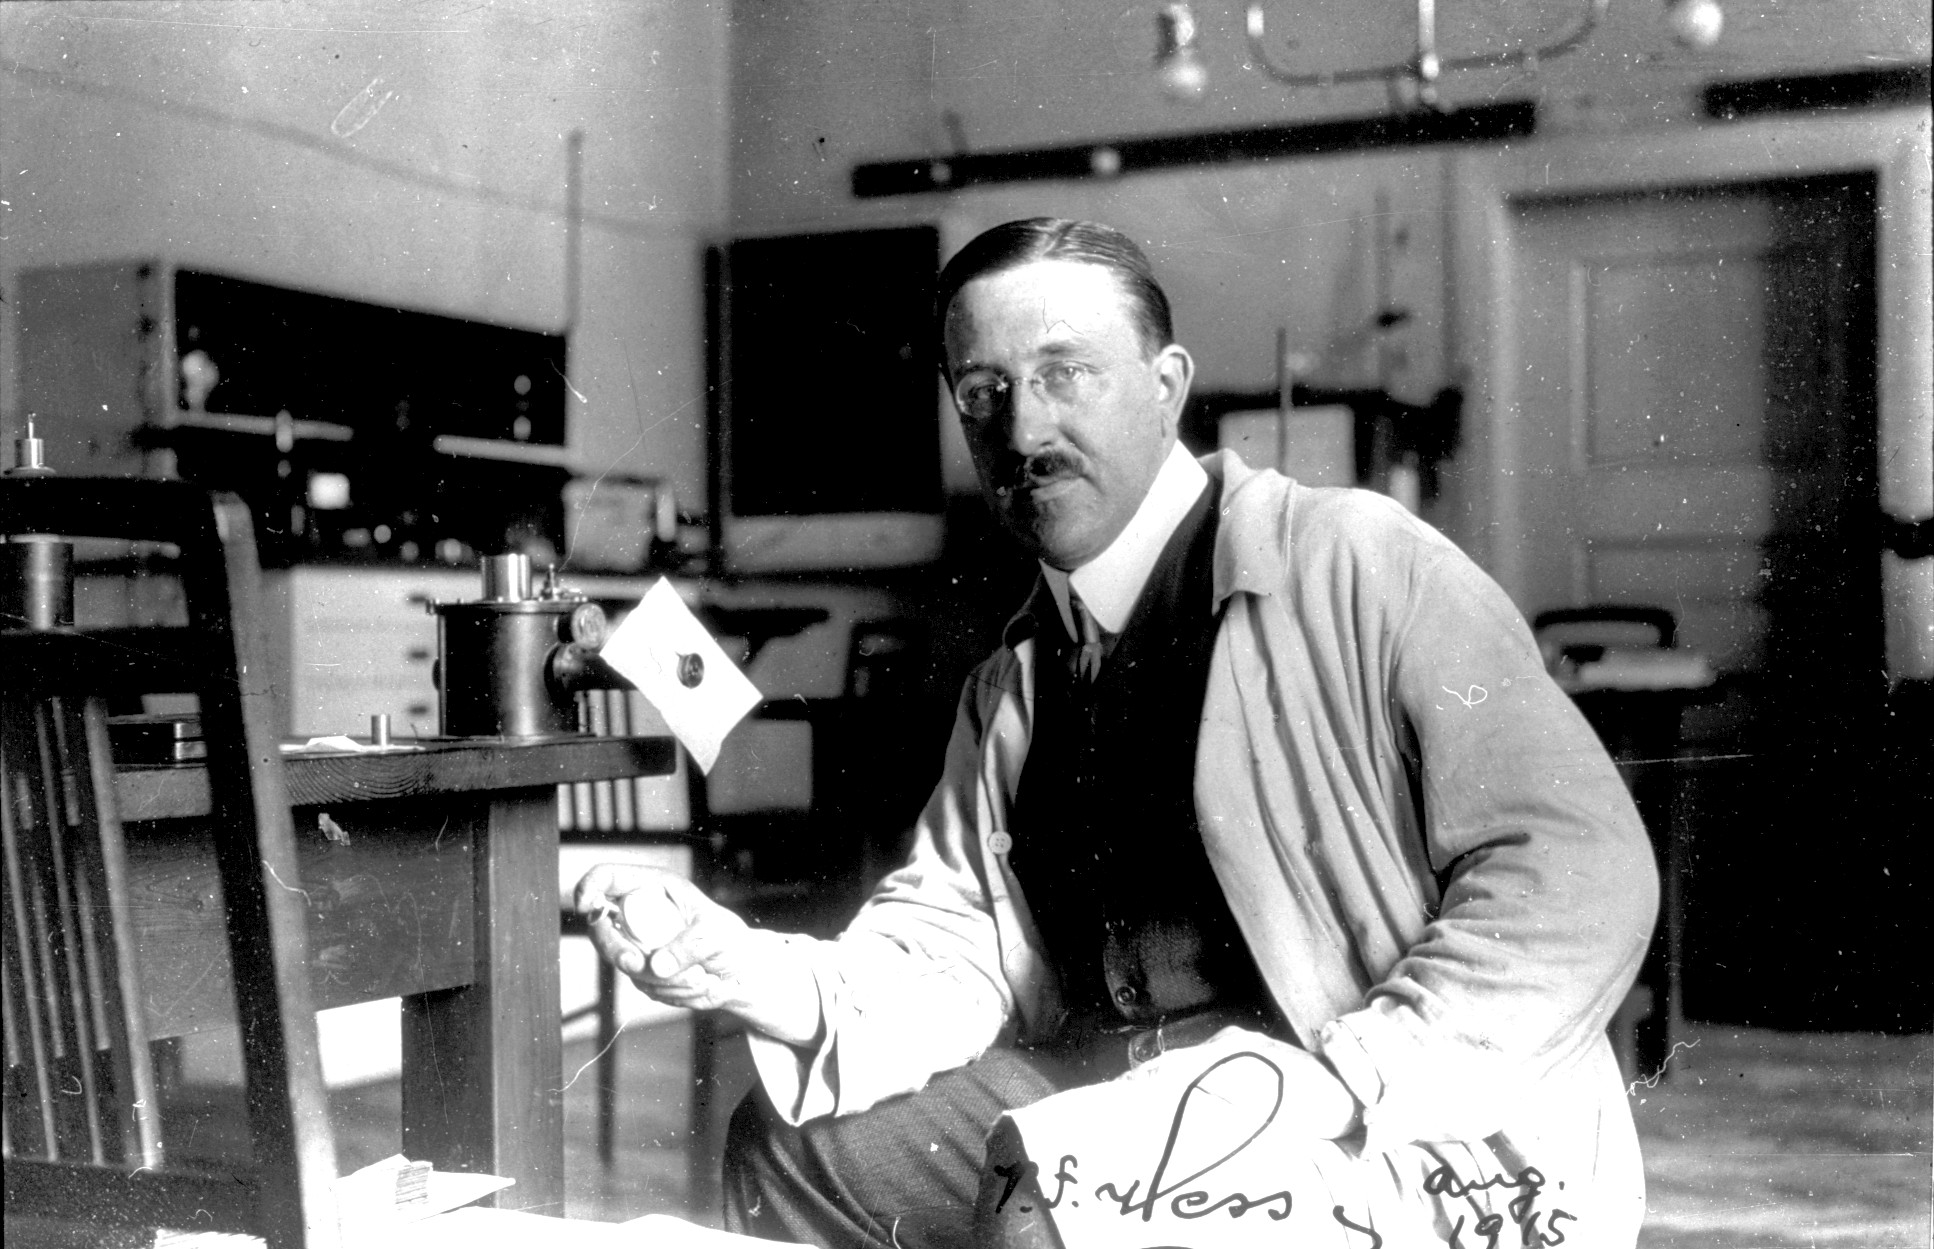
\includegraphics[width=\linewidth]{images/X-HESS-2140.jpg}
          \caption{Viktor Hess im Jahre 1915 \cite{hess}}
      \end{figure}
  \end{columns}
\end{frame}


\begin{frame}{}
  \begin{columns}
    \column{0.5\textwidth}
      \begin{itemize}
        \setlength\itemsep{0.5em}
        \item \textbf{1911}: Erste Ballonflüge durch Hess 1911 ($h \approx \SI{1000}{\metre}$)
        \item [$\rightarrow$] Bestätigung der Resultate von Gockel
        \item \textbf{1912, erste Hälfte}: Sechs weitere Ballonflüge, zu verschiedenen Tagszeiten ($h \lesssim \SI{2100}{\metre}$)
        \item [$\rightarrow$] Keine Korrelation der Ionsationrate mit Sonnenaktivitäten
        \item [$\rightarrow$] Bestätigung: Ionisatonsrate nimmt nicht signifikant stark mit der Distanz zur Erde ab
      \end{itemize}
        \vspace*{10px}

    Ziel von Hess: Untersuchung der Ionsationsrate in größeren Höhen
  
    \column{0.5\textwidth}
      \begin{figure}
          \centering
          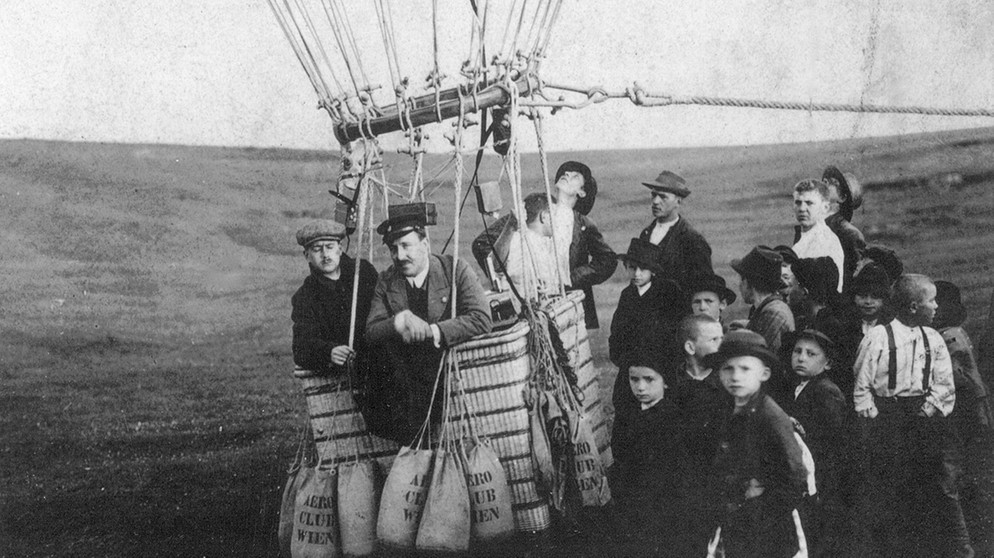
\includegraphics[width=\linewidth]{images/ballon.jpg}
          \caption{Victor Hess in einem Ballon um 1912 \cite{baloon}}
      \end{figure}
  \end{columns}
\end{frame}


\begin{frame}{}
  \begin{columns}
    \column{0.5\textwidth}
      \begin{itemize}
        \setlength\itemsep{0.5em}
        \item \textbf{7. August 1912}: Ballonflug von Hess auf bis zu $h \approx \SI{5350}{\metre}$
        \item [$\rightarrow$] Gemessener Anstieg der Ionisationsrate von $h \approx \SI{3000}{\metre}$ auf $h \approx \SI{5200}{\metre}$ um Faktor vier!
        \item [$\rightarrow$] Hess: Es muss sich um eine durchgringende Strahlung handeln, die die Atmosphäre von oben trifft (und nicht von der Sonne stammt)
        \item \textbf{1913, 1914}: Bestätigung der Ergebnisse, Ballonflüge von Werner Kolhörster ($h \approx \SI{9300}{\metre}$)
      \end{itemize}


      \begin{itemize}
        \item Anfangs bestand bei vielen Forschern Zweifel, dass die entdeckte Strahlung tatsächlich kosmischen Ursprunges war
      \end{itemize}

    \column{0.5\textwidth}

      \begin{figure}
          \centering
          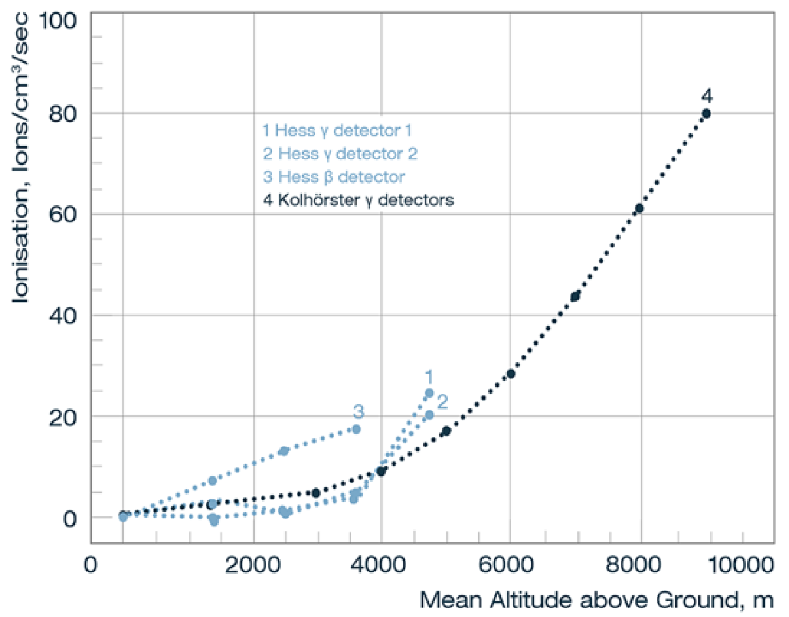
\includegraphics[width=\linewidth]{images/walter2.png}
          \caption{Ergebnisse des siebten Ballonfluges von Hess und des Ballonfluges von Kolhörster \cite{Hess:2018twh}}
      \end{figure}
  \end{columns}
\end{frame}


% Wenn mir ein gutes Bild zu den Folien über den Weg läuft...
%\begin{frame}{Die Identifikation als Teilchenstrahlung}
%  \begin{columns}
%    \column{0.5\textwidth}
%      \begin{itemize}
%        \setlength\itemsep{0.5em}
%        \item Große Durchdringtiefe der kosmischen Strahlung $\Rightarrow$ Identifikation als \gamma-Strahlung
%        \item Kolhörster: Absorptionskoeffizient der kosmischen Strahlung in Luft um Faktor \num{4.4} kleiner als Koeffizient von bekannten radioaktiven Quellen  
%        \item [$\rightarrow$] Härteres Spektrum?
%        \item Andere experimentelle Methoden lösten Elektrometer ab:
%        \item [$\rightarrow$] Nebelkammer (1911, Wilson)
%        \item [$\rightarrow$] Geiger-Müller-Zählrohr (1928, Geiger, Müller)
%      \end{itemize}
%  
%    \column{0.5\textwidth}
%      \begin{figure}
%          \centering
%          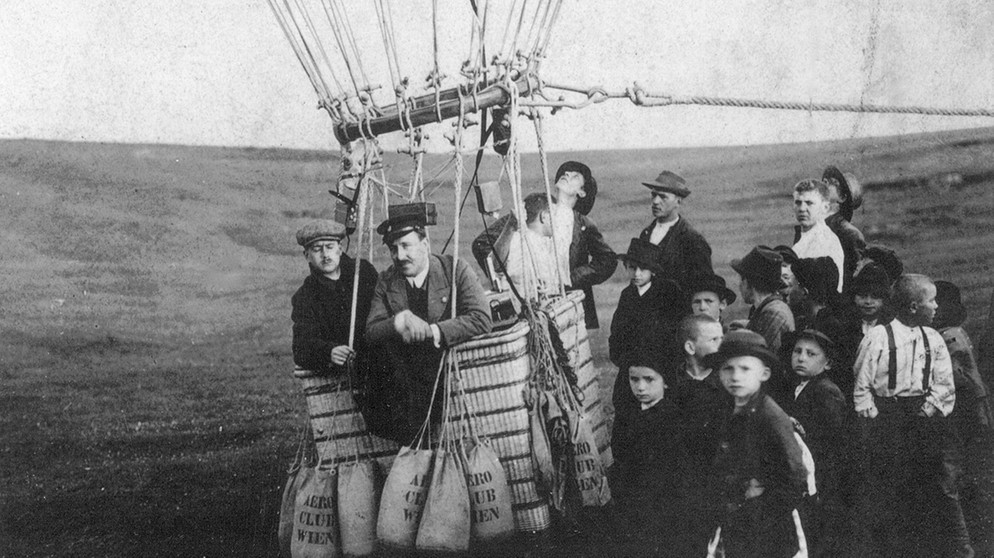
\includegraphics[width=\linewidth]{images/ballon.jpg}
%          \caption{Victor Hess in einem Ballon um 1912 \cite{baloon}}
%      \end{figure}
%  \end{columns}
%\end{frame}

\begin{frame}{Die Identifikation als Teilchenstrahlung}
      \begin{itemize}
        \setlength\itemsep{0.5em}
        \item Große Durchdringtiefe der kosmischen Strahlung $\Rightarrow$ Identifikation als \gamma-Strahlung
        \item Kolhörster: Absorptionskoeffizient der kosmischen Strahlung in Luft um Faktor \num{4.4} kleiner als Koeffizient von bekannten radioaktiven Quellen  
        \item [$\rightarrow$] Härteres Spektrum?
        \item Andere experimentelle Methoden lösten Elektrometer ab:
        \item [$\rightarrow$] Nebelkammer (1911, Wilson)
        \item [$\rightarrow$] Geiger-Müller-Zählrohr (1928, Geiger, Müller), Möglichkeit von Koinzidenzmessungen!
      \end{itemize}
\end{frame}


\begin{frame}{Die Identifikation als Teilchenstrahlung - Bothe und Kolhörster}
  \begin{columns}
    \column{0.5\textwidth}
      \begin{itemize}
        \setlength\itemsep{0.5em}
        \item \textbf{1929}: Koinzidenzmessungen von Bothe und Kolhörster mit Geiger-Müller-Zählrohren
        \item [$\rightarrow$] Ziel: Nachweis dass kosmische Strahlung aus \gamma-Strahlung besteht
        \item [$\rightarrow$] Idee: \gamma-Strahlung lösen Elektronen aus, welche beide Koinzidenzen durchqueren
        \item [$\rightarrow$] Beobachte Einfluss eines Absorbers auf die Koinzidenzen
      \end{itemize}
        \vspace*{10px}
  
    \column{0.5\textwidth}
      \begin{figure}
          \centering
          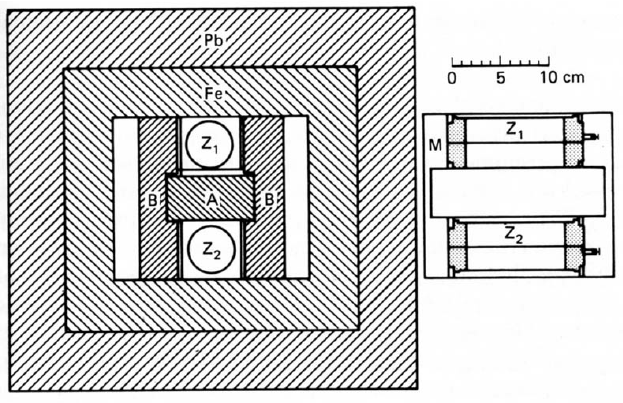
\includegraphics[width=\linewidth]{images/The-experiment-of-Bothe-and-Kolhoerster-in-Ref-48-Coincidences-between-counters-Z-1.png}
          \caption{Experiment von Bothe und Kolhörster \cite{ko}}
      \end{figure}
  \end{columns}
\end{frame}

\begin{frame}{Die Identifikation als Teilchenstrahlung - Bothe und Kolhörster}
  \begin{columns}
    \column{0.5\textwidth}
      \begin{itemize}
        \setlength\itemsep{0.5em}
        \item Mit \SI{4}{\centi\meter} Goldbarren konnten entgegen der Erwartung nur \SI{25}{\percent} der Koinzidenzen entfernt werden
        \item [$\rightarrow$] Die detektierten Teilchen sind so durchdringend wie die kosmische Strahlung selbst
        \item [$\rightarrow$] Es kann sich nicht um \gamma-Strahlung handeln sondern um geladene Teilchen!
      \end{itemize}
        \vspace*{10px}
  
    \column{0.5\textwidth}
      \begin{figure}
          \centering
          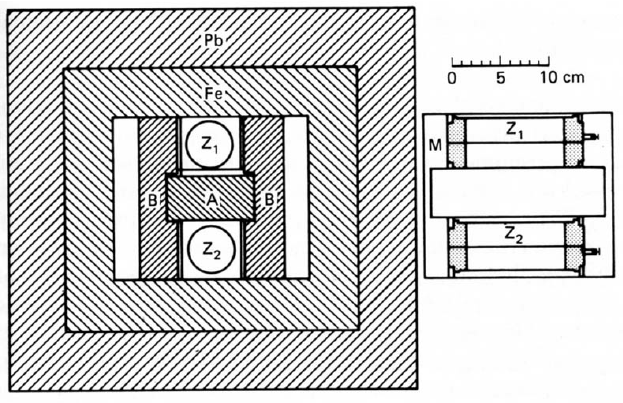
\includegraphics[width=\linewidth]{images/The-experiment-of-Bothe-and-Kolhoerster-in-Ref-48-Coincidences-between-counters-Z-1.png}
          \caption{Experiment von Bothe und Kolhörster \cite{ko}}
      \end{figure}
  \end{columns}
\end{frame}

\begin{frame}{Die Identifikation als Teilchenstrahlung - Breitengradeffekt}
  \begin{columns}
    \column{0.5\textwidth}
      \begin{itemize}
        \setlength\itemsep{0.5em}
        \item \textbf{1919}: Kolhörster: Erster Vorschlag, die Breitengradabhängigkeit der Ionisationsrate zu untersuchen
        \item \textbf{1932, 1933}: Nachweis der Abhängigkeit der Intensität der kosmischen Strahlung vom Breitengrad
        \item [$\rightarrow$] Intensität folgt dem geomagnetischen Feld
        \item [$\rightarrow$] Eindeutiger Nachweis, dass kosmische Strahlung aus geladenen Teilchen besteht
      \end{itemize}
        \vspace*{10px}
  
    \column{0.5\textwidth}
      \begin{figure}
          \centering
          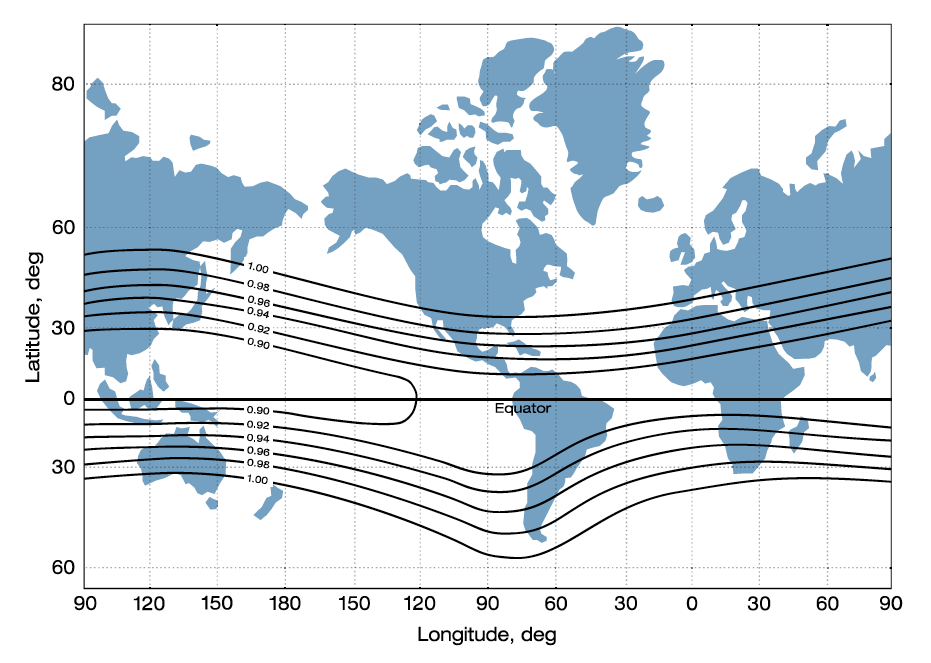
\includegraphics[width=\linewidth]{images/scrrenshot}
          \caption{Breitengradabhängigkeit der kosmischen Strahlung \cite{9789400754225}}
      \end{figure}
  \end{columns}
\end{frame}


\begin{frame}{Teilchenphysikalische Entdeckungen - Positron}
  \begin{columns}
    \column{0.5\textwidth}
      \begin{itemize}
        \setlength\itemsep{0.5em}
        \item \textbf{1931}: Carl Anderson: Untersuchung der kosmischen Strahlung über eine Nebelkammer mit starkem Magnetfeld
        \item[$\rightarrow$] Entdeckung von positiv geladenen Teilchen
        \item \textbf{August 1932}: Weitere Untersuchungen mit \SI{6}{\milli\meter} Bleiplatte (Flugrichtung)
        \item[$\rightarrow$] Eindeutiger Nachweis des Positrons

      \end{itemize}
        \vspace*{10px}
  
    \column{0.5\textwidth}
      \begin{figure}
          \centering
          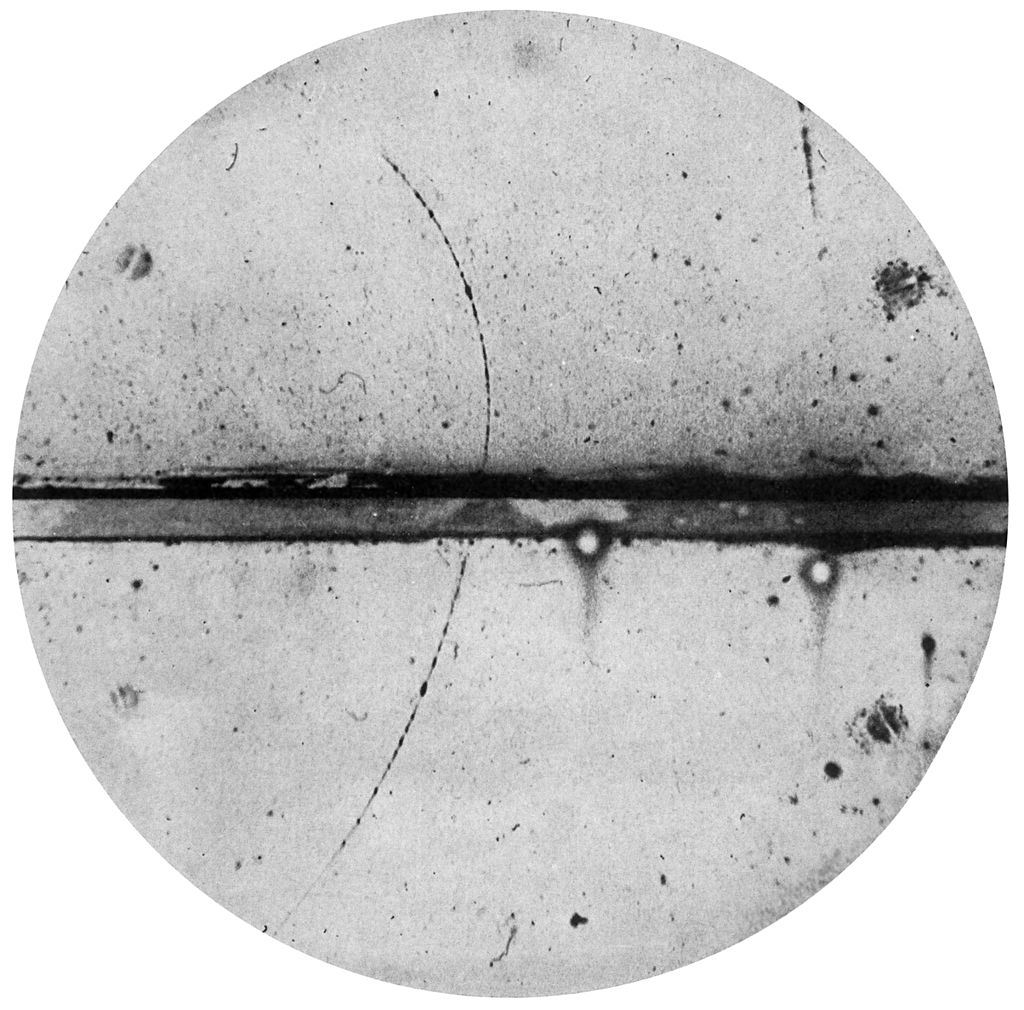
\includegraphics[width=0.7\linewidth]{images/positron.jpg}
          \caption{Nebelkammeraufnahme des ersten entdeckten Positrons, publiziert 1933 \cite{positron}}
      \end{figure}
  \end{columns}
\end{frame}

\begin{frame}{Teilchenphysikalische Entdeckungen - Myon und Pion}

      \begin{itemize}
        \setlength\itemsep{0.5em}
        \item \textbf{1934}: Anderson: Entdeckung von Teilchenspuren in Nebelkammern mit deutlich geringerer Absorption als Elektronen aber kleinerer Masse als Protonen
        \item \textbf{1937}: Neddermeyer, Anderson: Nach genaueren Untersuchungen Bekanntgabe der Entdeckung eines neuen Teilchens (Myon)
        \item \textbf{1947}: Perkins, erster Nachweis von Pionen in der Höhenstrahlung (Yukawa-Teilchen)
        \item \textbf{1948}: Bestimmung der Lebensdauer der geladenen Pionen, erstmals über Beschleunigerexperiment
      \end{itemize}

\end{frame}


%%%% TEIL 2 %%%%

\begin{frame}{Entdeckung Teilchenschauer}
  \begin{columns}
    \column{0.45\textwidth}
      \begin{itemize}
        \setlength\itemsep{0.5em}
        \item \textbf{1933}: Experiment von Rossi\item[$\rightarrow$]
        Nutzung von drei in Koinzidenz geschalteten Geiger-Müller-Zählern
        \item[$\rightarrow$] Absorber oberhalb von Experiment
        \item Ergebnis: Bei Verdickung des Absorbers zunächst vergrößerung der Koinzidenzrate, erst danach Abnahme
        \item Interpretation Rossi: Erzeugung von Sekundärteilchen durch kosmische Strahlung wenn diese den Absorber treffen
      \end{itemize}
        \vspace*{10px}
  
    \column{0.55\textwidth}
      \begin{figure}
          \centering
          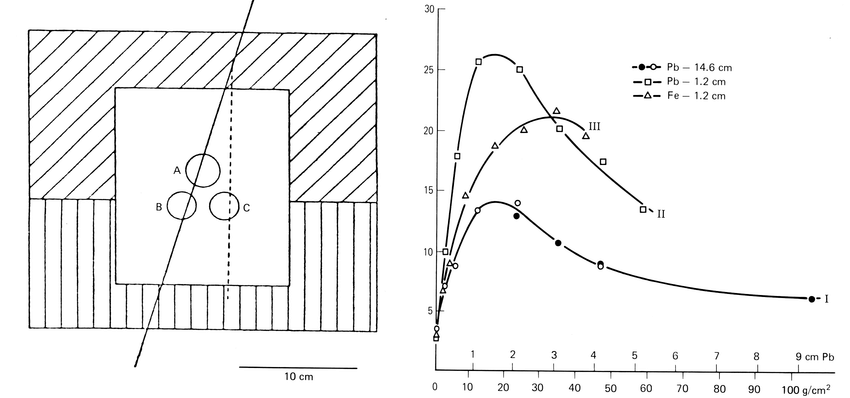
\includegraphics[width=\linewidth]{images/Rossis-transition-curve-The-experiment-in-which-the-abundant-production-of-secondary.png}
          \caption{Experiment von Rossi (1933) zur Entdeckung von Teilchenschauern \cite{9789400754225}}
      \end{figure}
  \end{columns}
\end{frame}

\begin{frame}{Entdeckung Teilchenschauer}
  \begin{columns}
    \column{0.5\textwidth}
      \begin{itemize}
        \setlength\itemsep{0.5em}
        \item \textbf{1938}: Schmeiser und Bothe vermuten, dass Rossis Beobachtung auch "Luftschauer" impliziert
        \item \textbf{1938}: Schmeiser, Kolhörster: Messung von Koinzidenzen von zwei Geigerzählern in Abhängigkeit ihres Abstandes
        \item \textbf{1939}: Auger: Ebenfalls abstandsabhängige Messung der Koinzidenzen
        \item[$\Rightarrow$] Schätzung der Primärenergie durch Auger auf \SI{e15}{\electronvolt}!
      \end{itemize}
        \vspace*{10px}
  
    \column{0.5\textwidth}
      \begin{figure}
          \centering
          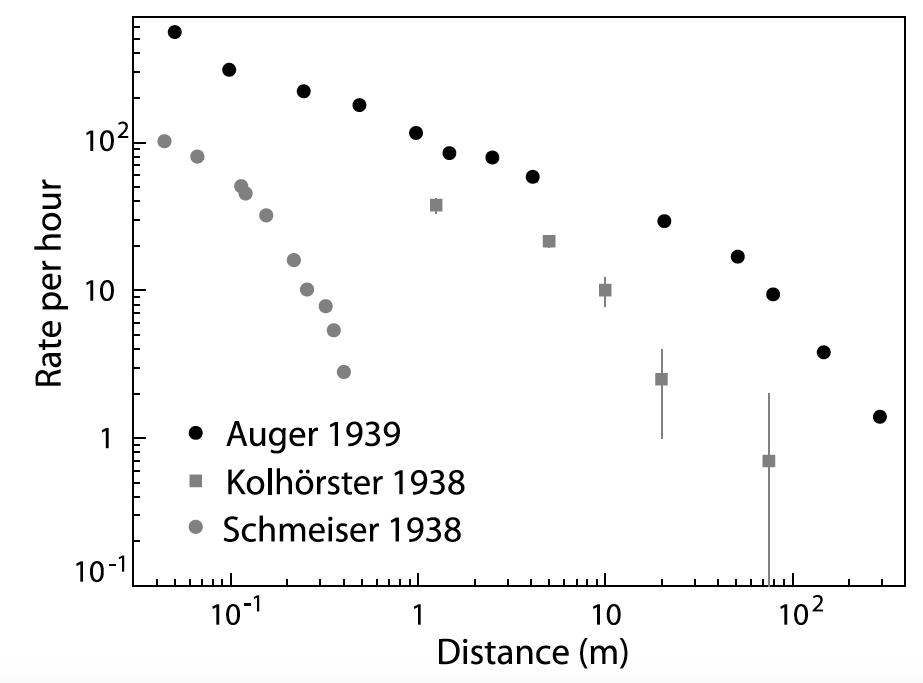
\includegraphics[width=\linewidth]{images/auger_messung.png}
          \caption{Experiment von Rossi (1933) zur Entdeckung von Teilchenschauern \cite{9789400754225}}
      \end{figure}
  \end{columns}
\end{frame}



% Finde ich nicht gut :-(
%\begin{frame}{Entdeckung Teilchenschauer}
%  \begin{columns}
%    \column{0.5\textwidth}
%      \begin{itemize}
%        \setlength\itemsep{0.5em}
%        \item Seit den späten 30er Jahren: Theoretisches Verständnis, dass Schauer eine hadronische, myonische und eine elektromagnetische Komponente besitzt
%        \item Erste Schauerexperimente unter Nutzung von Geigerzählern
%        \item[$\rightarrow$] Erste Experimente mit Durchmesser $d \approx \SI{10}{\metre}$ zur Untersuchung von Energien im Bereich \SI{e14}{\electronvolt} bis \SI{e16}{\electronvolt}
%        \item[$\rightarrow$] 1950er Jahre: Array aus Geigerzählern mit einer Fläche von \SI{0.6}{\kilo\metre\squared} (Großbritannien)
%      \end{itemize}
%        \vspace*{10px}
%  
%    \column{0.5\textwidth}
%      \begin{figure}
%          \centering
%          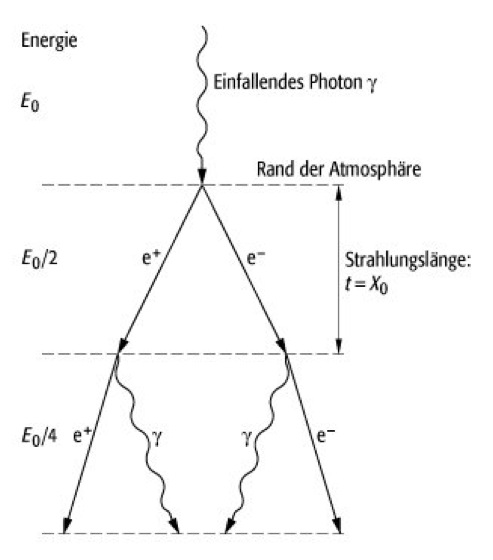
\includegraphics[width=0.7\linewidth]{images/fff12451_w.jpg}
%          \caption{Heitler Modell zur Beschreibung elektromagnetischer Schauer \cite{heitler}}
%      \end{figure}
%  \end{columns}
%\end{frame}

\begin{frame}{Erste Schauerexperimente}
  \begin{columns}
    \column{0.5\textwidth}
      \begin{itemize}
        \setlength\itemsep{0.5em}
        \item Durchführung erster Beobachtungen unter Nutzung von Geigerzählern
        \item[$\rightarrow$] Experimente der Größenordnung $d \approx \SI{10}{\metre}$ zur Untersuchung von Primärteilchenenergien \SI{e14}{\electronvolt} bis \SI{e16}{\electronvolt}
        \item \textbf{$\approx$ 1950}: Entwicklung von Szintillatoren ermöglichen, zusammen mit Photomultipliern, Nutzung zur Schauerdetektion
        \item[$\rightarrow$] \textbf{1954 bis 1957}: "Agassiz Astronomical Station", Harvard
        \item \textbf{1959}: Entdeckung des "Knies" im kosmischen Spektrum (\SI{e15}{\electronvolt}) in Russland
      \end{itemize}
        \vspace*{10px}
  
    \column{0.5\textwidth}
      \begin{figure}
          \centering
          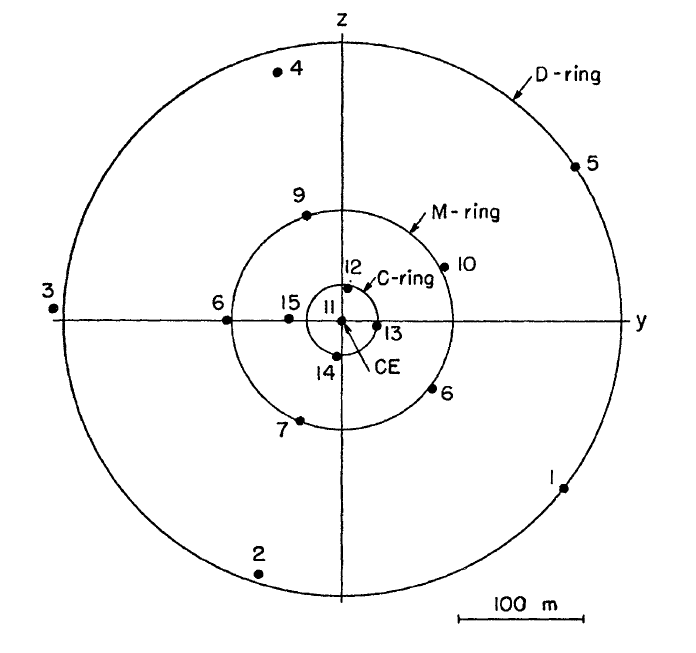
\includegraphics[width=0.7\linewidth]{images/AGASSIZ}
          \caption{Schematische Anordnung des Agassiz Arrays, Nutzung von 15 Szintillatoren \cite{9789400754225}}
      \end{figure}
  \end{columns}
\end{frame}

\begin{frame}{}
  \begin{columns}
    \column{0.4\textwidth}
      \begin{itemize}
        \setlength\itemsep{0.5em}
        \item \textbf{1958}: Porter: Langfristige Unterdrückung des bakteriellen Wachstums im Wasser
        \item[$\rightarrow$] Ermöglichte die Nutzung stabiler Wasser-Čerenkov-Detektoren
        \item Prinzipieller Aufbau der Detektoren bis heute identisch
      \end{itemize}
        \vspace*{10px}
  
    \column{0.6\textwidth}
      \begin{figure}
          \centering
          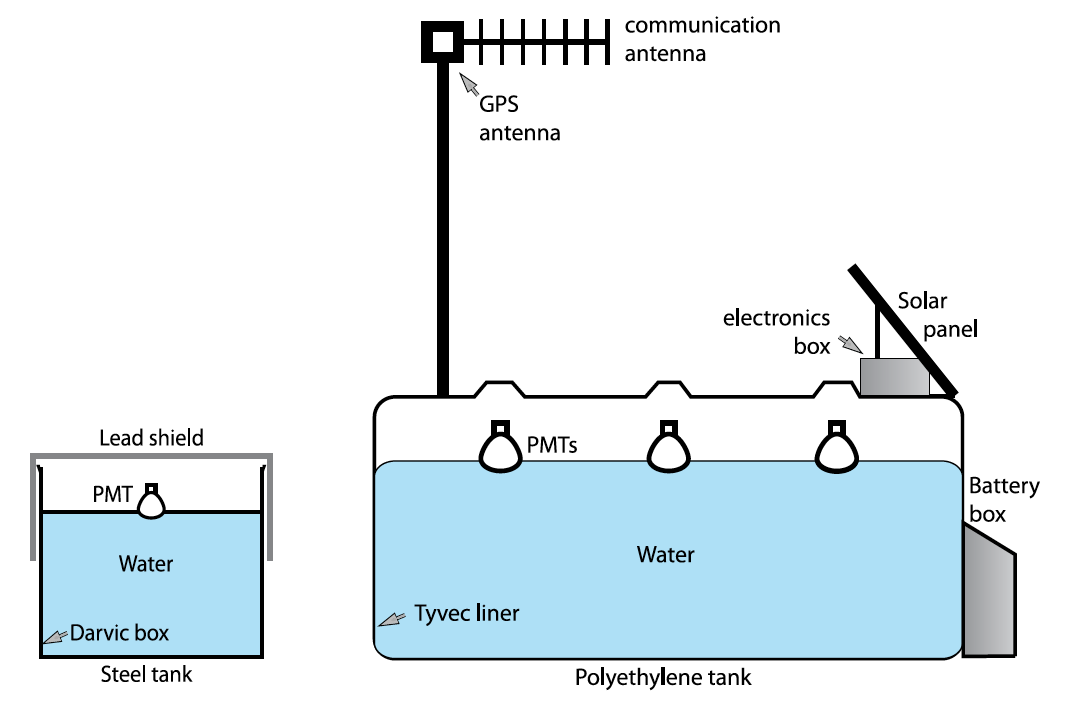
\includegraphics[width=\linewidth]{images/cherenkov}
          \caption{Links: Wasser-Čerenkov-Detektoren nach Porter. Rechts: Protoyp der Wasser-Čerenkov-Detektoren von Pierre Auger \cite{9789400754225}.}
      \end{figure}
  \end{columns}
\end{frame}

\begin{frame}{}
  \begin{columns}
    \column{0.5\textwidth}
      \begin{itemize}
        \setlength\itemsep{0.5em}
        \item Große Forschritte beim Verständnis von Luftschauern durch die Arbeitsgruppe rund um Bruno Rossi am MIT
        \item[$\rightarrow$] Entwicklung neuer Analysemethoden
        \item \textbf{1959}: Bau des Volcano Ranch Arrays (New Mexico) durch John Linsley (MIT)
        \item[$\rightarrow$] Erstes (von 7) erbauten Arrays mit einer Fläche von mehr als \SI{1}{\kilo\metre\squared}
        \item[$\rightarrow$] 19 Plastikszintillatoren (je \SI{3.3}{\metre\squared}) mit PMT's
        \item[$\rightarrow$] Erste Messung von Ereignissen über \SI{e18}{\electronvolt}
        \item[$\rightarrow$] \textbf{1963}: Erste Hinweise auf den "Ankle" bei \SI{e18}{\electronvolt}
      \end{itemize}
        \vspace*{10px}
  
    \column{0.5\textwidth}
      \begin{figure}
          \centering
          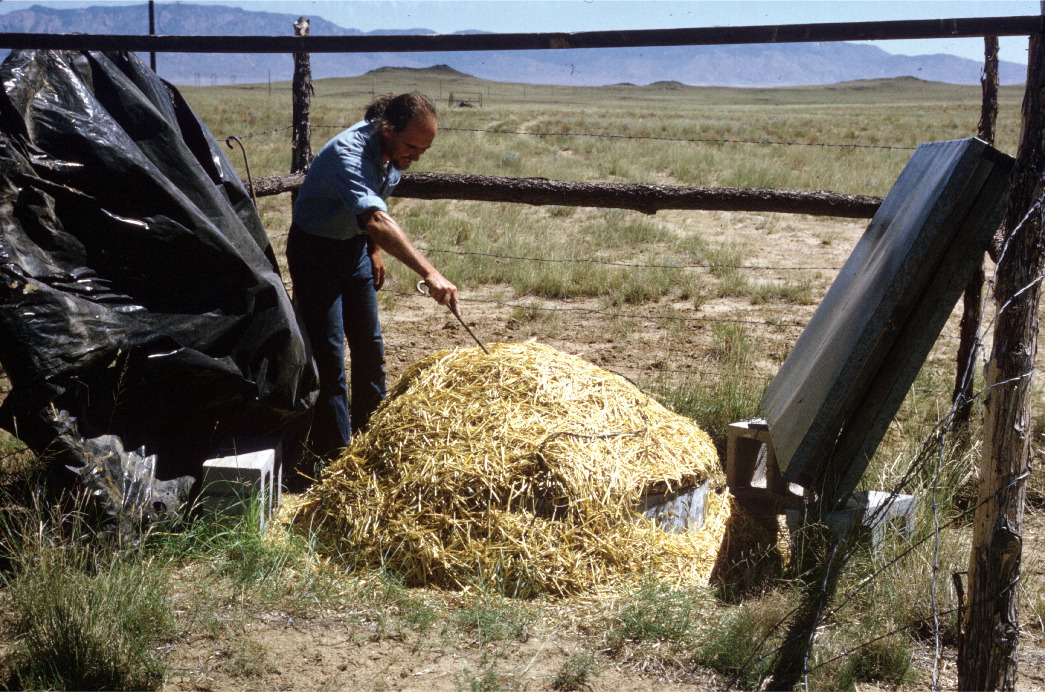
\includegraphics[width=\linewidth]{images/linsey.jpg}
          \caption{John Linsey am Volcano Ranch Experiment auf der Suche nach Klapperschlangen \cite{linsey}}
      \end{figure}
  \end{columns}
\end{frame}


\begin{frame}{Entdeckung des CMB}
  \begin{columns}
    \column{0.6\textwidth}
      \begin{itemize}
        \setlength\itemsep{0.5em}
        \item \textbf{1965}: Entdeckung des kosmischen Mikrowellenhintergrundes (Penzias, Wilson)
      	\item \textbf{1966}: Hinweis auf eine mögliche Abschwächung des Spektrums durch Wechselwirkung von Protonen mit CMB-Photonen (Greisen, Zatsepin, Kuzmin $\rightarrow$ GZK-Effekt)
      	\item Planung für mehrere riesige Arrays begann bereits vor der CMB-Entdeckung
      	\item[$\rightarrow$] Trotzdem sollte keines der zu diesen Zeitpunkt geplanten Arrays groß genug sein um den Effekt des GZK-Cutoffs eindeutig zu bestätigen oder zu widerlegen
      \end{itemize}
        \vspace*{10px}
  
    \column{0.4\textwidth}
      \begin{figure}
          \centering
          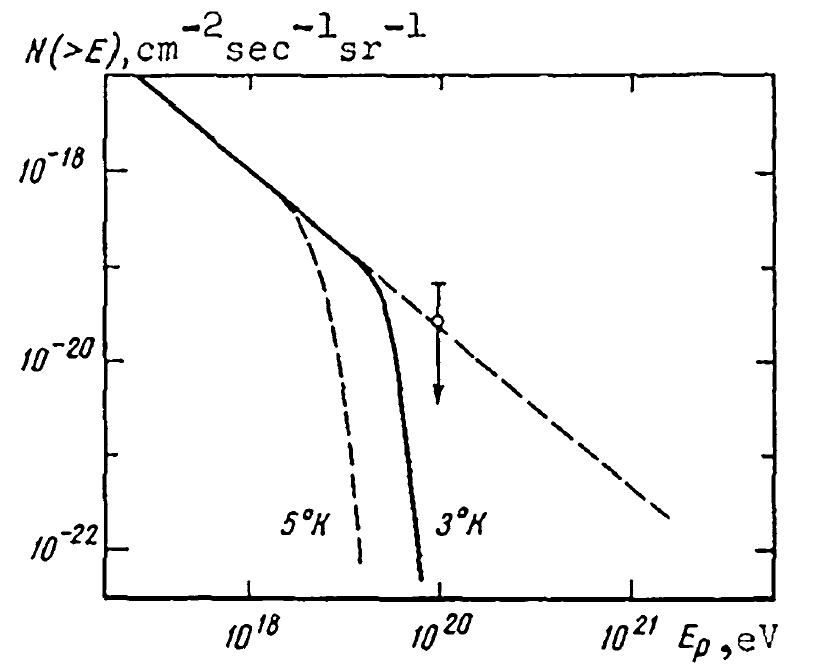
\includegraphics[width=\linewidth]{images/gzk}
          \caption{Vorhersage des GZK-Cutoffs nach Zatsepin und Kuzmin (1966) \cite{9789400754225}}
      \end{figure}
  \end{columns}
\end{frame}


\begin{frame}{Weitere Experimente...}
      \begin{itemize}
        \setlength\itemsep{0.5em}
        \item \textbf{1964 bis 1987}: Haverah Park experiment, Großbritannien (\SI{12}{\kilo\metre\squared})
        \item[$\rightarrow$] Wasser-Čerenkov-Detektoren und Myondetektoren
        \item \textbf{1970 bis heute}: Yakutsk Array, Sibirien (\SI{18}{\kilo\metre\squared})
        \item[$\rightarrow$] Messung Čerenkovlicht in der Luft
        \item \textbf{1968 bis 1979}: The Sydney University Giant Air Shower Recorder (SUGAR) (\SI{70}{\kilo\metre\squared})
        \item[$\rightarrow$] 54 Wasserszintilatoren unter der Erde
        \item[$\rightarrow$] Erstmals wurden die einzelnen Messstationen autonom betrieben!
        \item[$\rightarrow$] Erste Messungen eines Arrays dieser Größe in der südlichen Hemisphäre
        \item \textbf{1990 bis 2004}: Akeno Giant Air Shower Array (AGASA), Japan (\SI{100}{\kilo\metre\squared})
        \item[$\rightarrow$] 111 Szintilatordetektoren
        \item[$\rightarrow$] Messung von 11 Ereignissen über \SI{e20}{\electronvolt} (kein Anzeichen eine Cutoffs)


      \end{itemize}
\end{frame}


\begin{frame}{}
  \begin{columns}
    \column{0.5\textwidth}
      \begin{itemize}
        \setlength\itemsep{0.5em}
        \item \textbf{1969}: Erstmals erfolgreiche Detektion von Luftschauern durch Fluoreszenzlicht in der Luft in Japan
        \item \textbf{$\approx$ 1970} Beginn des Baus eines großen Luft-Fluoreszenz-Detektors ("Fly's Eye")
        \item[$\rightarrow$] 67 "Augen", je \SI{1.5}{\meter} Spiegel zur Überwachung eines $\SI{5}{\degree} \times \SI{5}{\degree}$ Teil des Himmels
        \item \textbf{1986}: Betriebsbeginn von "Fly's Eye II", \SI{3.4}{\kilo\metre} entfernt um stereoskopische Aufnahmen durchführen zu können
        \item \textbf{1991}: Aufnahme eines Teilchens mit einer Energie von \SI{3.2e20}{\electronvolt} (OMG-Teilchen)

      \end{itemize}
        \vspace*{10px}
  
    \column{0.5\textwidth}
      \begin{figure}
          \centering
          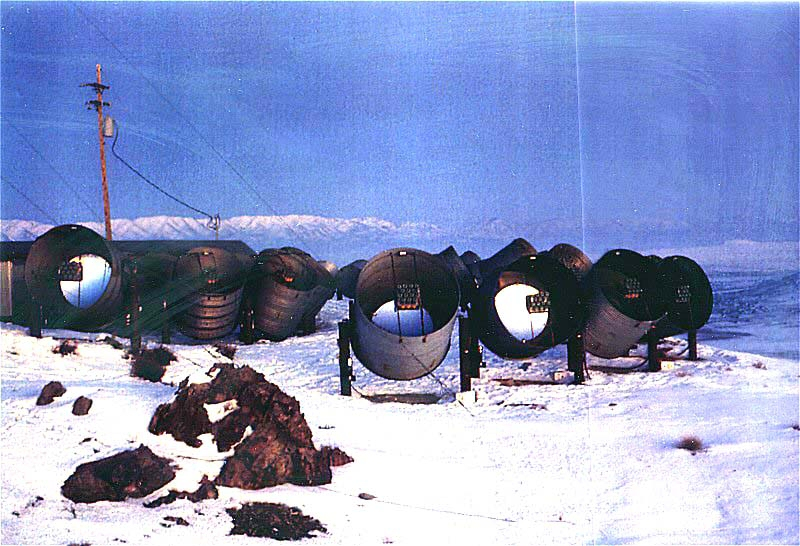
\includegraphics[width=\linewidth]{images/FlysEye.jpg}
          \caption{Detektor "Fly's Eye" in der Wüste von Utah \cite{flyeye}}
      \end{figure}
  \end{columns}
\end{frame}

\begin{frame}{}
TODO:
      \begin{itemize}
        \item Cygnus X-3 und das Kiel Array
        \item Als Beispiel für daraus resultierende Experimente: KASCADE (und damit verbunden kurz der Grund für die Entwicklung von CORSICA)
        \item Pierre Auger: Geschichte (Cronin, GZK-Cutoff)
      \end{itemize}

\end{frame}

\appendix

\begin{frame}[allowframebreaks]{Quellen}
	\printbibliography

\end{frame}

\end{document}
